\documentclass[11pt, letterpaper]{article}

% ABNT %
\usepackage[brazil]{babel}
\usepackage[utf8]{inputenc}
\usepackage[margin=1in]{geometry}
% FIGURAS %
\usepackage{graphicx}
\usepackage{fancyhdr}
\usepackage{setspace}
\usepackage{subfig}
\usepackage{float}
\usepackage{fancyref}
%
\usepackage{placeins}
\renewcommand{\contentsname}{Sumário}
%------------------------------------------------------
\begin{document}
\begin{titlepage}
\thispagestyle{empty}
\parbox{1.5cm}{
\includegraphics[scale=0.25]{logo_uerj_cinza.png}}
\vspace*{-0.8cm}{\hspace*{1.5cm} \Large{\textbf{Universidade do Estado do Rio de Janeiro}\\
\hspace*{5.3cm}}}
\Large{Departamento de Física Teórica} \\

\vspace{5cm}
\hspace{3.0cm} \Large{\textbf{Medidas de tempo de queda de um objeto\\}}
\hspace*{4.5cm} \Large{\textbf{e Estimativa para gravidade no local\\}}
\vspace{8cm}

\begin{flushright}
Aluno: José Gonçalves Chaves Junior \\
M:202020477411\\
Curso: Física \\
Prof: Antonio Vilela
\end{flushright}

\end{titlepage}
%-----------------------------------------------------------------
\tableofcontents

\newpage
\listoftables
\newpage
%-----------------------------------------------------------------
\section{Introdução}
%-----------------------------------------------------------------
Desde os tempos mais remotos, o homem estuda os movimentos que ocorrem na natureza. Aristóteles, filósofo grego, acreditava que, se abandonássemos dois corpos de massas diferentes, de uma mesma altura, o corpo mais pesado tocaria o solo primeiro, ou seja, o tempo de queda desses corpos seriam diferentes. \\
Essa crença perdurou por muito tempo, até a chegada do século XVII. Ao introduzir o método experimental, Galileu Galilei chegou à conclusão de que dois corpos de massas diferentes, quando desprezada a resistencia do ar e abandonados da mesma altura, alcançam o solo no mesmo instante, e podemos perceber isso através da função horária: \\
$$ H(t) = H_{0} + v_{0}t + \frac{1}{2}gt^2 $$

Dessa equação, podemos isolar g: \\
\textbf{$$g = \frac{2(H - H_{0} - v_{0}t)}{t^2}$$} \\
Como sabemos H, Ho,t, e como o objeto parte do repouso, finalmente teremos: \\

$$ g = \frac{2H}{t^2} $$

Dessa forma, vemos que o tempo de queda contribui para a aceleração do corpo, não a massa (nesse caso). Desprezando a resistência do ar, dois objetos de massas diferentes quando abandonados do repouso chegam ao mesmo tempo ao solo pois estão sob influência da mesma aceleração (g).

%----------------------------------------------------------------
\section{Objetivo}
%----------------------------------------------------------------

Neste Experimento, o objetivo é estimar o tempo de queda de um objeto e após o procedimento, estimar o módulo da gravidade no local do experimento e verificar se o resultado é compatível ou não com o valor de referência g = 9,787899 m.s^{-2}.


%----------------------------------------------------------------
\section{Procedimento Experimental}
%----------------------------------------------------------------
Para realizar o experimento, foi usado:
\begin{enumerate}
\item Uma trena ( 3 $\pm$ 0,01 m);
\item Uma borracha de látex (6 cm x 2 cm) ;  
\item Caneta Esferográfica de cor Azul (15cm x 0,5cm x 0,5 cm);
\item Cronômetro do celular com marcação na ordem dos ms; \\

De início, a trena foi usada para medir 1,80 m a partir do solo e marcar um ponto na parede, para ser o ponto inicial da queda. Logo após a marcação, a borracha foi solta da altura, mediu-se 60 vezes seu tempo de queda, e, após a coleta, os dados foram analisados para estimar o tempo de queda.
\newpage
%----------------------------------------------------------------
\section{Análise dos Dados Coletados}
%----------------------------------------------------------------
%valores coletados
\FloatBarrier
\begin{table}[!ht]
\centering
\begin{tabular}{|l|l|1|1|} 
\hline
- & t(s) & -  & t(s)\\
\hline
1 & 0,50 & 16 & 0,61\\
\hline
 2 & 0,61 & 17 & 0,56\\
\hline
 3 & 0,58 & 18 & 0,51\\
\hline
 4 & 0,60 &  19 & 0,57\\
\hline
 5 & 0,59 & 20 & 0,65\\
\hline
 6 & 0,62 &  21 & 0,63\\
\hline
 7 & 0,57 & 22 & 0,62\\
\hline
 8 & 0,58 & 23 & 0,60\\
\hline
 9 & 0,62 & 24 & 0,65\\
\hline
 10 & 0,60 & 25 & 0,57\\
 \hline
 11 & 0,64 & 26 & 0,63\\
 \hline
 12 & 0,60 & 27 & 0,55\\
 \hline
 13 & 0,60 & 28 & 0,68\\
 \hline
 14 & 0,54 & 29 & 0,63\\
 \hline
 15 & 0,57 & 30 & 0,55\\
\hline
\end{tabular}
\caption{Dados coletados nas 30 primeiras medições do tempo de queda}
\end{table}
\FloatBarrier
%table1
\begin{table}[!ht]
\centering
\begin{tabular}{|l|l|1|1|}
\hline
- & t(s) & -  & t(s)\\
\hline
31 & 0,55 & 46 & 0,65\\
\hline
 32 & 0,63 & 47 & 0,66\\
\hline
 33 & 0,63 & 48 & 0,63\\
\hline
 34 & 0,67 & 49 & 0,67\\
\hline
 35 & 0,67 & 50 & 0,68\\
\hline
 36 & 0,66 &  51 & 0,66\\
\hline
 37 & 0,65 & 52 & 0,61\\
\hline
 38 & 0,63 & 53 & 0,62\\
\hline
 39 & 0,62 &  54 & 0,61\\
\hline
 40 & 0,57 & 55 & 0,60\\
 \hline
 41 & 0,51 & 56 & 0,66\\
 \hline
 42 & 0,58 & 57 & 0,65\\
 \hline
 43 & 0,65 & 58 & 0,62\\
 \hline
 44 & 0,67 & 59 & 0,60\\
 \hline
 45 & 0,58 & 60 & 0,62\\
\hline
\end{tabular}
\caption{Dados coletados nas últimas 30  medições do tempo de queda.}
\end{table}
\newpage
%-------------------------------------%
\begin{figure}[!htbp]
\centering
\begin{tabular}{11}
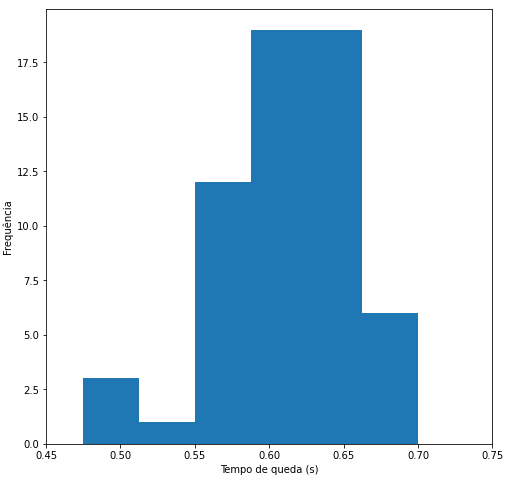
\includegraphics[width=0.5\textwidth]{hist_0.png} &
 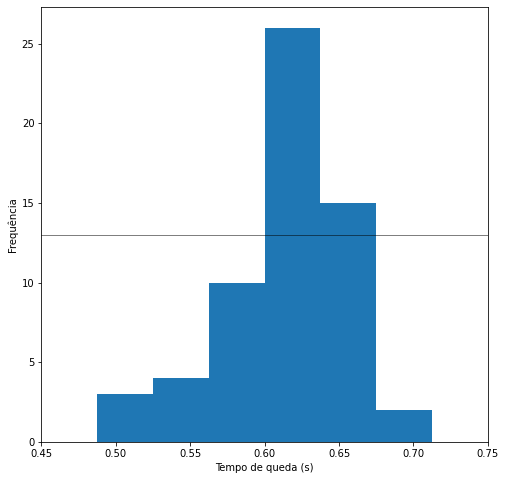
\includegraphics[width=0.5\textwidth]{hist_2.png}
 \\
 (a) Histograma das 60 medidas & (b) Histograma com largura a meia altura*
\end{tabular}
\caption{Histogramas das medições.}
\end{figure}
\textbf{* - Largura a meia altura: 0.075}\\
\textbf{* - Valor a meia altura: 13.0}
\FloatBarrier
\begin{table}[!ht]
\centering
\begin{tabular}{|l|l|}
\hline
Valor Máximo & Intervalo\\
\hline
  26.0 & (0.6, 0.638)\\
\hline
\end{tabular}
\caption{Valor máximo e intervalo do valor máximo do Histograma (b).}
\end{table}
%-----------------------------%
\FloatBarrier
\begin{table}[!ht]
\centering
\begin{tabular}{|l|l|}
\hline
Valor Mínimo & Intervalo\\
\hline
  0.0 & (0.45,0.75)\\
\hline
\end{tabular}
\caption{Valor mínimo e intervalo do valor máximo do Histograma (b).}
\end{table}
%----------------------------------------------------&
\newpage
%média e desvio padrão%
\FloatBarrier
\begin{table}[!ht]
\centering
\begin{tabular}{|1|l|}
\hline
- & t(s)\\
\hline
Média & 0,612  \\
\hline
Desvio Padrão & 0,043\\
\hline
\end{tabular}
\caption{Média e Desvio Padrão das medições.}
\end{table}
%----------------------------
%--------------------------
\FloatBarrier
\begin{table}[!ht]
\centering
\begin{tabular}{|l|l|}
\hline
Incerteza Estatística (s) & Erro da Média* (s) \\
\hline
  0.005 & 0.011\\
\hline
\end{tabular}
\caption{Incertezas das medições.}
\end{table}

\textbf{* - O erro da média foi calculado através do erro instrumental de 0,01 m recomendado pela $Prof.^{a}$ Maria de Fátima no roteiro, e calculado a partir da soma em quadratura dos erros.} 
%-------------------------
\subsection{Estimativas finais para o tempo de queda}
%------------------------------------
\FloatBarrier
\caption{Estimativa final para o tempo de queda da borracha.}
\centering
\begin{tabular}{|l|}
\hline
 \textbf{t = (0,61 $\pm$ 0,01) s} \\
\hline
\end{tabular}
\caption{Estimativa final para o tempo de queda da borracha.}
\end{table}
\begin{figure}[!htbp]
\centering
\begin{tabular}{1}
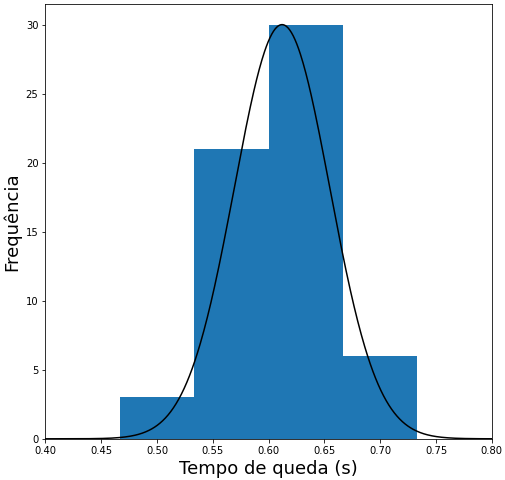
\includegraphics[width=0.4959\textwidth]{gaus_1.png}
 \\
\end{tabular}
\caption{Distribuição Gaussiana do valor do tempo de queda encontrado.}
\end{figure}
%-------------------------------------
\newpage
\section{Estimativas para gravidade}
Para estimarmos o valor da gravidade, utilizaremos as equações: 


\begin{equation}
g = \frac{2H}{média^{2}_{t}} \pm \sigma_{g}
\end{equation}
onde , $$ \sigma_{g} = \sqrt{(\frac{\sigma_{g}}{\sigma{t}})^{2}.\sigma_{t}} = 0,36 m.s^{-2}.$ \\
Além de considerármos H constante e igual à 1,80m e o valor de \textbf{t} ser igual à \textbf{\textit{$média_{t}$}}, temos que $$\frac{\sigma_{g}}{\sigma_{t}} = \frac{-4H}{média^{3}_{t}}$$ \\
 teremos como valor final:\\
 \begin{equation}
 g = (9,61 \pm 0,36) m.s^{-2}.
  \end{equation}
\section{Compatibilidade}
Com os nossos resultados, podemos verificar a compatibilidade destes, com o valor referência g = 9,787899 m.s^{-2}. 
% compatibilidade
\FloatBarrier
\begin{table}[!ht]
\centering
\begin{tabular}{|1|1|}
\hline
Discrepância & 0,176 m.s^{2} \\
\hline
Erro Relativo & 0,037 \\
\hline
Erro Percentual & 3,73 \%\\
\hline 
\end{tabular}
\caption{Dados para a compatibilidade com o valor referência.}
\end{table}
%---------------

\begin{figure}[!htbp]
\centering
\begin{tabular}{1}
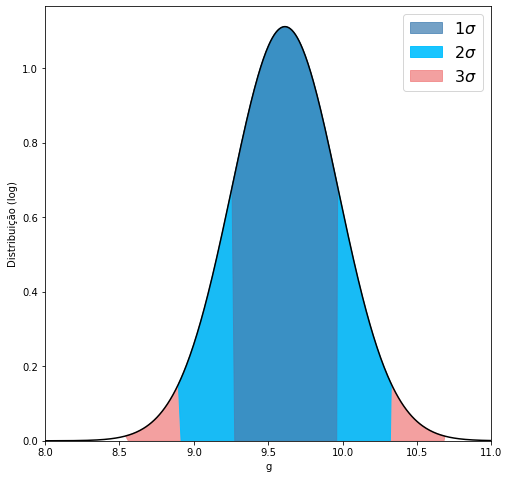
\includegraphics[width=0.5\textwidth]{gaus_2.png}
 \\
\end{tabular}
\caption{Intervalo de confiança do valor de g encontrado.}
\end{figure}
\newpage
\section{Conclusão}
Para sabermos se o resultado é compatível ou não, basta calcularmos a razão
\begin{equation}
r = \frac{\vert g_{ref} - g_{exp}\vert}{\sigma_{g}} = 0,4911
\end{equation}
Portanto, por $r \leq 2$, podemos afirmar que o valor é compatível com o referente, o que pode ser evidenciado pela Figura 3.
\newpage
\subsection{Respostas}
\textbf{1}- A última medição que fiz foi para medir a mesa do meu quarto. Os experimentos realizados no laboratório contribuiram bastante para que eu tivesse sucesso na medição, como queria movê-la de lugar no meu escritório, e por este ser pequeno, foi necessário medir com bastante atenção (não só para não ser um esforço em vão, mas para que funcionasse), e funcionou! \\
\textbf{2}- Através das incertezas, podemos ter uma base melhor para analisar, ou seja, podemos antes de realizar algum trabalho, analisar se é válido ou não.\\
\textbf{3}- Por mais que os \textbf{Histogramas (a) e (b)} apresentem intervalos com uma alta amplitude, quando olhamos a \textbf{Figura 2} podemos ver que a função ficou bem distribuída, e o valor médio se encontra realmente numa região de maior "frequência".\\
\textbf{4}- Não foi o que eu esperava. Talvez por não ter uma bolinha ou uma esfera maçica em casa, o formato do objeto pode ter contribuído pela discrepância. Entretanto, o valor encontrado satisfaz, mesmo assim, quando comparadado com o tempo previsto; inclusive, com o mesmo erro da média.\\
\newpage
\section{Bibliografia}
 Ref. 1: https://brasilescola.uol.com.br/fisica/queda-livre.htm ; \\
 Ref. 2: https://querobolsa.com.br/enem/fisica/queda-livre-e-lancamento-vertical ; \\ 
 Ref. 3: \textit{“Estimativas e erros em experimentos de Física”}, coleção Comenius, 3a
 Edição. Ed UERJ. \\

\end{document}

